\documentclass{article}
\usepackage[left=2cm,right=2cm,top=2cm,bottom=2cm]{geometry}
\usepackage{multicol}
\usepackage{graphicx}
\usepackage{amssymb}
\usepackage{amsmath}
\usepackage{mathtools}
\usepackage[hidelinks]{hyperref}
\usepackage{tocloft}

\usepackage{latex4ei/scientific}

\title{Elektronische Schaltungen: Interaktives Cheatsheet}
\author{Paul Thiel, Justus Rossmeier}

%\RequirePackage{latex4ei/latex4ei_unicode}

\newcommand{\jw}{\j\omega}

% set font
\renewcommand{\familydefault}{\sfdefault}

% -- begin custom TOC for circuits
\newcommand{\listcircuitname}{Liste der Schaltungen (anklicken zum hinspringen)}
\newlistof{circuit}{cir}{}
\newenvironment{circuit}[2]{%
	\refstepcounter{circuit}
	% Content in TOC
	\addcontentsline{cir}{circuit}{%
		\parbox[c][\linewidth + 3\baselineskip][c]{\linewidth}{%
			\parbox[c][\linewidth][c]{\linewidth}{%
				\begin{center}
					\includegraphics[width=\linewidth,height=\linewidth,keepaspectratio]{#2}
				\end{center}
			}
			\parbox[c][3\baselineskip][t]{\linewidth}{%
				\begin{flushleft}
					#1\hfill
				\end{flushleft}
			}
		}
	}
	% Content on page
	\section{#1}
	\begin{minipage}[t]{12em}
		\ \vspace{-\baselineskip}\\
		\includegraphics[height=16em,width=\linewidth,keepaspectratio]{#2}\\
		\hyperref[listofcircuits]{\bfseries\small(zurück zur Liste)}
	\end{minipage}
	\begin{minipage}[t]{\linewidth - 12em}
}{%
	\end{minipage}
}

\renewcommand{\cftdotsep}{\cftnodots}

\let\mylistofcircuit\listofcircuit
\renewcommand{\listofcircuit}{%
	\subsection*{\listcircuitname}
	\label{listofcircuits}
	\vspace{-1.5em}
	\begin{multicols}{4}
		\mylistofcircuit
	\end{multicols}
}
% -- end

\cftpagenumbersoff{circuit}

% DOCUMENT_BEGIN ===============================================================
\begin{document}
\IfFileExists{git.id}{\input{git.id}}{}
\ifdefined\GitRevision\mydate{\GitNiceDate\ (git \GitRevision)}\fi

% Title (needs ./img/Logo.pdf)
\maketitle

\listofcircuit
\pagebreak

\begin{circuit}{Stromspiegel mit Widerstand}{img/stromspiegel-mit-widerstand.pdf}
Annahme: Sättigung $\rightarrow V_{\ir GS1} = V_{\ir DD}-RI_{\ir IN}$\\
Überprüfe, ob Annahme korrekt\\
$\frac{I_{\ir out}}{I_{\ir in}} = \frac{(W/L)_2}{(W/L)_1}$
\end{circuit}
\begin{circuit}{Schalter (Transmission-Gate)}{img/transmission-gate.pdf}
$V_{\ir out} \approx V_{\ir in} \rightarrow$ Transistoren in Triodenbereich\\
\end{circuit}
\begin{circuit}{Transistor mit resistiver Last (Source an GND, immer +)}{img/transistor-mit-resistiver-last-1.pdf}
	%TODO ESB
	Verstärkung: $\frac{V_{\ir out}}{V_{\ir in}} = g_{\ir m1}(r_{\ir DS1}\parallel R_D)$\\
	$r_{\ir out} = r_{\ir DS1}\parallel R_D$\\
\end{circuit}
\begin{circuit}{Transistor mit resistiver Last ($V_{\ir in}$ an Source)}{img/transistor-mit-resistiver-last-2.pdf}	
	$A \approx g_mR_d$\\
	$r_\text{out} = r_{DS} \parallel R_D \approx R_D$\\
	$r_{\ir in} = R_D \frac{r_{\ir DS}\parallel \frac{1}{g_m}}{r_{\ir DS}\parallel R_D}$
	
\end{circuit}
\begin{circuit}{Transistor mit resistiver Last ($R_S$ an Source)}{img/transistor-mit-resistiver-last-3.pdf}	
	%TODO
	
\end{circuit}
\begin{circuit}{Sourceschaltung mit Stromquelle (- - -)}{img/sourceschaltung-mit-stromquelle.pdf}
%TODO ESB
Verstärkung: $\frac{V_{\ir out}}{V_{\ir in}} = -g_{\ir m1}r_{\ir DS1}$\\
$r_{\ir out} = r_{\ir DS1}$
\end{circuit}
\begin{circuit}{Sourceschaltung mit aktiver Last (- -)}{img/sourceschaltung-mit-aktiver-last.pdf}
%TODO ESB
Verstärkung: $\frac{V_{\ir out}}{V_{\ir in}} = -g_{\ir m1}(r_{\ir DS1}\parallel r_{\ir DS2})$\\
$r_{\ir out} = r_{\ir DS1}\parallel r_{\ir DS2}$
\end{circuit}
\begin{circuit}{Sourceschaltung mit Diodenlast [$V_{\ir in}$ am unteren Transistor (-)]}{img/sourceschaltung-mit-diodenlast-1.pdf}
	%TODO ESB
	Verstärkung: $\frac{V_{\ir out}}{V_{\ir in}} = -g_{\ir m1}\left( r_{\ir DS1}\parallel r_{\ir DS2}\parallel \frac{1}{g_{\ir m2}}\right)$\\
	$r_{\ir out} = r_{\ir DS1}\parallel r_{\ir DS2}\parallel \frac{1}{g_{\ir m2}}$
\end{circuit}
\begin{circuit}{Sourceschaltung mit Diodenlast [$V_{\ir in}$ am oberen Transistor]}{img/sourceschaltung-mit-diodenlast-2.pdf}
%TODO
\end{circuit}
\begin{circuit}{Drainschaltung mit aktiver Last [ohne $C_L$ ($\approx 1$)]}{img/drainschaltung-mit-aktiver-Last-1.pdf}
	Verstärkung: $\frac{V_{\ir out}}{V_{\ir in}} = \frac{g_{\ir m1}(r_{\ir DS1}\parallel r_{\ir DS2})}{1 + g_{\ir m1}(r_{\ir DS1}\parallel r_{\ir DS2})}$ (kann auch $<1$ sein)\\
	$r_{\ir out} = \frac{r_{\ir DS1}\parallel r_{\ir DS2}}{1 + g_{\ir m1}(r_{\ir DS1}\parallel r_{\ir DS2})}$
\end{circuit}
\begin{circuit}{Drainschaltung mit aktiver Last [mit $C_L$]}{img/drainschaltung-mit-aktiver-Last-2.pdf}
	%TODO ESB
	Verstärkung: $A(\omega) = \frac{g_{\ir m1}(r_{\ir DS1}\parallel r_{\ir DS2})}{1 + g_{\ir m1}(r_{\ir DS1}\parallel r_{\ir DS2})+\j\omega C_L(r_{\ir DS1}\parallel r_{\ir DS2})}$\\
	Näherung: $\frac{g_{\ir m1}}{g_{\ir m1}+\j\omega C_L}$\\
	Betrag: $\abs{A(\omega)} = \frac{1}{\sqrt{1+(\omega C_L / g_{\ir m1})^2}}$\\
	Phase: $\phi(A(\omega) = \arctan{(-\omega C_L / g_{\ir m1})}$\\

%\end{circuit}
%\begin{circuit}{Differenzstufe mit Stromspiegel-Last (pMOS)}{img/differenzstufe-mit-stromspiegel-last-1.pdf}

\end{circuit}
\begin{circuit}{Differenzstufe mit Diodenlast}{img/differenzstufe-mit-diodenlast.pdf}
$A \approx -\frac{g_{m1}}{g_{m2}}$\\
$r_{out}=r_{DS1}\parallel r_{DS2}\parallel \frac{1}{g_{m2}} \approx \frac{1}{g_{m2}}$

\end{circuit}
\begin{circuit}{Stromspiegel mit Stromquelle}{img/stromspiegel-mit-stromquelle.pdf}
$I_\text{out} = I_\text{in}\frac{W_2}{L_2}\frac{L_1}{W_1}$\\
$r_\text{in} = r_\text{DS1} \parallel \frac{1}{g_{m1}} \approx \frac{1}{g_{m1}}$\\
$r_\text{out} = r_\text{DS2}$\\

\end{circuit}
\begin{circuit}{Differenzstufe mit resistiver Last}{img/differenzstufe-mit-resistiver-last.pdf}
$A_\text{diff} = -g_\text{m1}(r_\text{DS1}\parallel R_\text{D})\approx -g_mR_D$\\
$A_\text{cm} = -\frac{R_\text{D}}{2r_\text{ds0}}$\\
Bedingung für Sättigungsbereich:\\
$V_\text{GS1} + V_\text{GS3} - V_\text{th} \leq V_\text{in} \leq V_\text{out-} + V_\text{th}$


\end{circuit}
\begin{circuit}{Differenzstufe mit Stromspiegel-Last (nMOS)}{img/differenzstufe-mit-stromspiegel-last-2.pdf}
%TODO
\end{circuit}
\begin{circuit}{Differenzstufe mit Diodenlast}{img/differenzstufe-mit-diodenlast.pdf}
%TODO
\end{circuit}

\begin{circuit}{Spannungsfolger mit Lastwiderstand}{img/spannungsfolger-mit-lastwiderstand.pdf}
	$V_{\ir in} \geq V_{\ir GS3}-V_{\ir th}$\\
	$V_{\ir in} \leq V_{\ir DD} - V_{\ir GS7} - V_{\ir GS1} + V_{\ir th}$\\
	$V_{\ir out} \geq V_{\ir GS5} - V_{\ir th}$\\
	$V_{\ir out} \leq V_{\ir DD} - V_{\ir GS6} + V_{\ir th}$\\
	\\
	$R_L > \frac{V_{\ir out}}{I_{\ir D6}}$\\
	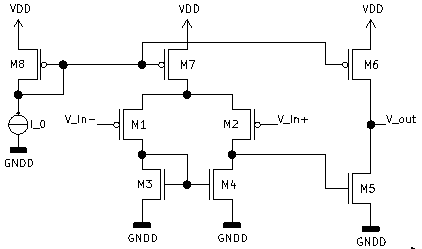
\includegraphics{img/op-innenleben.pdf}
\end{circuit}

\begin{circuit}{Invertierender Verstärker}{img/invertierender-verstärker.pdf}
%TODO ESB
Verstärkung (ideal): $A = -\frac{R_2}{R_1}$\\
Verstärkung (real): $A = -\frac{A\frac{R_2}{R_1+R_2}}{1+A\frac{R_1}{R_1+R_2}}$\\
Ausgangswiderstand: $r_{\ir out} = 0$\\
Eingangswiderstand: $r_{\ir in} = R_1$\\

\end{circuit}
\begin{circuit}{Invertierender Verstärker mit Offset}{img/invertierender-verstärker-mit-offset.pdf}
	Ausgangsspannung (ideal): $-\frac{R_2}{R_1}V_{\ir in}+\left( 1+\frac{R_2}{R_1}\right)V_{\ir os}$\\
	Ausgangsspannung (real): $-\frac{A\frac{R_2}{R_1+R_2}}{1+A\frac{R_1}{R_1+R_2}}V_{\ir in}+\frac{A}{1+A\frac{R_1}{R_1+R_2}}V_{\ir os}$


\end{circuit}
\begin{circuit}{Nichtinvertierender Verstärker}{img/nichtinvertierender-verstärker.pdf}
\subsection{$V_{\ir ref} = 0$}
Verstärkung (ideal): $A = 1 + \frac{R_2}{R_1}$\\
Verstärkung (real): $A = \frac{A}{1+A\frac{R_1}{R_1+R_2}}$\\
Ausgangswiderstand: $r_{\ir out} = 0$\\
Eingangswiderstand: $r_{\ir in} = \infty$\\
\subsection{$V_{\ir ref} \neq 0$}
$A=\frac{V_{\ir out,max}-V_{\ir ref}}{V_{\ir in}-V_{\ir ref}}$


\end{circuit}
\begin{circuit}{Summierverstärker}{img/summierverstärker.pdf}
Ausgangsspannung: $V_{\ir out} = - \sum_{k=1}^N V{\ir ein,k}\frac{R_3}{R_k}$\\
Fall $k=2$: $-\left( \frac{V_{\ir in,1}}{R_1} + \frac{V_{\ir in,2}}{R_2}R_3\right)$\\ 
Verstärkung (real): $A = \frac{A}{1+A\frac{R_1}{R_1+R_2}}$\\
Ausgangswiderstand: $r_{\ir out} = 0$\\
Eingangswiderstand: $r_{\ir in} = \infty$\\

\end{circuit}
\begin{circuit}{Differenzverstärker}{img/differenzverstärker.pdf}
Ausgangsspannung: $V_{\ir out} = V_{\ir in,p}\frac{R_4}{R_3+R_4} \frac{R_1+R_2}{R_1} - \frac{R_2}{R_1} V_{\ir in,p}$\\
Fall $R_3 = R_4$ und $R_1 = R_2$: $V_{\ir out} = V_{\ir in,p} - V_{\ir in,p}$

\end{circuit}
\begin{circuit}{Strom/Spannungswandler}{img/strom-spannungswandler.pdf}
	$V_ {\ir out} = V_{\ir ref}+I_{\ir in}R_2$
\end{circuit}
\begin{circuit}{Instrumentenverstärker mit 2 OPV}{img/instrumentenverstärker-mit-2-op.pdf}
	$V_{\ir O} = \left(1+\frac{R_2}{R_1}+\frac{2R_2}{R_5}\right)(V_{\ir i2} - V_{\ir i1})$
\end{circuit}

\begin{circuit}{Operationsverstärker}{img/op-innenleben.pdf}
	Verstärkung Diff: $A_{\ir diff} = -g_{\ir m1}(r_{\ir DS2}\parallel r_{\ir DS4})$\\
	Verstärkung Ausgang: $A_{\ir ausgang} = -g_{\ir m5}(r_{\ir DS5}\parallel r_{\ir DS6})$\\
	Verstärkung gesamt: $A = g_{\ir m1}(r_{\ir DS2}\parallel r_{\ir DS4})g_{\ir m5}(r_{\ir DS5}\parallel r_{\ir DS6})$
\end{circuit}


\begin{circuit}{Miller Operationsverstärker}{img/miller-op.pdf}
%TODO ESB
%TODO Spannungsfolger mit Lastwiderstand
Verstärkung Ausgangsstufe: $A = g_{\ir m5}(r_{\ir DS5}\parallel r_{\ir DS6})$
$C_1 = C_F(1+A) \approx C_FA$ \qquad $C_2 = C_F\left(1+\frac{1}{A}\right) \approx C_F$ \\
$C_{\ir out} = C_2 + C_L$\\
Grenzfrequenz: $f_{G1} = \frac{1}{2\pi C_1r_{\ir out,diff}}$ \quad $f_{G2} = \frac{1}{2\pi C_2r_{\ir out,ausgang}}$\\
$A_0 = g_{\ir m1}(r_{\ir DS2}\parallel r_{\ir DS4})g_{\ir m5}(r_{\ir DS5}\parallel r_{\ir DS6})$\\
Übertragungsfunktion: $A(\omega)=\frac{A_0}{\left(1+\j\frac{f}{f_1}\right)\left(1+\j\frac{f}{f_2}\right)}$\\

\end{circuit}
\begin{circuit}{Komparator}{img/komparator.pdf}
Schaltschwellen: $V_H = 1 + \frac{R_2}{R_1}V_{\ir th}$ \qquad $V_L = \left( 1 + \frac{R_2}{R_1}\right) V_{\ir th}-\frac{R_1}{R_2}V_{\ir DD}$\\
Hysterese: $V_{\ir HYS} = V_H - V_L = \frac{R_1}{R_2}V_{\ir DD}$
\end{circuit}

\begin{circuit}{Komperator mit Hysterese}{img/komparator-mit-hysterese.pdf}
	Obere Schwelle: $V_{\ir H}=\left(1+\frac{R_3}{R_4}\right)V_{\ir TH}$\\
	Untere Schwelle: $V_L = \left(1+\frac{R_3}{R_4}\right)V_{\ir TH}-\frac{R_3}{R_4}V_{\ir CC}$\\
	Hysterese: $V_{\ir HYS} = V_{\ir H}-V_{\ir L}$
\end{circuit}

\begin{circuit}{Invertierender Bandpass}{img/invertierender-bandpass.pdf}
	Übertragungsfunktion $H(\jw)=-\frac{Z_2(\jw)}{Z_1(\jw)}=-\frac{R_2}{R_1}\cdot\frac{\jw R_1C_1}{1+\jw R_1C_1}\cdot\frac{1}{1+\jw R_2C_2}$\\
	Grenzfrequenz Hochpass $\omega_1=\frac{1}{R_1C_1}$\\
	Grenzfrequenz Tiefpass $\omega_2=\frac{1}{R_2C_2}$
\end{circuit}

\begin{circuit}{Nicht-invertierender Verstärker mit part. Tiefpass}{img/nichtinvertierender-verstärker-mit-partiellem-tiefpass.pdf}
	Übertragungsfunktion $H(\jw)=1+\frac{R_2}{R_1}$ $\frac{1}{1+\jw CR_2} = 1+\frac{R_2}{R_1}\frac{1-\jw CR_2}{1+(\omega CR_2)^2}$\\
	Betrag: $\abs{H(\jw)}=1+\frac{R_2}{R_1}\frac{1}{\sqrt{1+(\omega CR_2)^2}}$\\
	Phase: $\phi(H(\jw)) = \arctan\left(-\frac{\omega CR_2}{\frac{R_1}{R_2}\left[1+(\omega CR_2)^2\right]+1 }\right)$\\
	Für kleine $\omega$: $H(\jw) \approx 1 + \frac{R_2}{R_1}$\\
	Für große $\omega$: $H(\jw) \approx 1$
\end{circuit}

\begin{circuit}{Nicht-invertierender Verstärker mit part. Hochpass}{img/nichtinvertierender-verstärker-mit-partiellem-hochpass.pdf}
	Übertragungsfunktion $H(\jw)=1+\frac{R_2}{R_1\parallel\left(R_3+\frac{1}{\jw C}\right)}$\\
	Für kleine $\omega$: $H(\jw) \approx 1+\frac{R_2}{R_1}$\\
	Für große $\omega$: $H(\jw) \approx 1+\frac{R_2}{R_1\parallel R_3}$
\end{circuit}

\begin{circuit}{CMOS Inverter}{img/cmos-inverter.pdf}
	Verstärkung: $A = - \frac{g_{\ir m1}+g_{\ir m2}}{ g_{\ir DS1}+ g_{\ir DS2}}$\\
	Ausgangswiderstand: $r_{\ir out} = \frac{1}{g_{\ir DS1}+ g_{\ir DS2}}$
\end{circuit}

\begin{circuit}{Sampler}{img/sampler.pdf}
	$V(t) = V_0\left[1-\exp(-\frac{t}{\tau})\right]$\\
	$\tau = (R_{\ir out}+R_{\ir on})C = \frac{1}{2\pi f_c}$\\
	Nyquist Prinzip: $f_{\ir sample} > 2f_{\ir signalBW}$
\end{circuit}

\begin{circuit}{Switched-capacitor Prinzip}{img/switched-capacitor}
	Zur Vermeidung von Schwankungen zwischen Widerständen\\
	Mittlerer Strom: $I_{\ir AB} = Qf_{\ir clk} = (V_{\ir in}-V{\ir out})Cf_{\ir clk}$\\
	Äquivalenter Widerstand: $R = \frac{V_{\ir in}-V_{\ir out}}{I_{\ir AB}} = \frac{1}{Cf_{\ir clk}}$
\end{circuit}

\begin{circuit}{AD Wandler}{img/ad-widerstand.pdf}
	Quantisierungsschritt: $\Delta = V_{\ir LSB} = \frac{V_{\ir ref}}{2^n}$\\
	Anzahl Komparatoren: $2^n-1$\\
	Unterreferenzwerte: $V_r = \frac{\text{Widerstandswert bis zur Referenz}}{\text{Gesamtwiderstand}}V_{\ir ref}$\\
	Quantisierungsschrittschawankung: $\Delta_{\ir meas} = V_{r_n+1}-V_{r_n}$\\
	Differentielle Nichtlinearität: $\text{DNL}(n) = \frac{\Delta_{\ir meas}-\Delta}{\Delta}$ \quad $\text{DNL}_{\ir spec} = \frac{\max{\abs{\Delta_{\ir meas}}}-\Delta}{\Delta}$\\
	Integrale Nichtlinearität: $\text{INL}(n) = (1+\text{GE})\sum_{i=1}^k \text{DNL}(i)$\\
	%TODO: GE??
\end{circuit}

\begin{circuit}{DA Wandler (Stromquellen)}{img/da-stromquellen.pdf}
	$V_{\ir out} = \frac{A}{1+A}\left(V_{\ir os}+\frac{RI}{8}(8b_1+4b_2+2b_3+b_4)\right)$\\
	Verstärkungsfehler: $GE = -\frac{1}{A}$\\
\end{circuit}

\begin{circuit}{DA Wandler (Widerstände)}{img/da-widerstand.pdf}
	$V_{\ir LSB = \frac{V_{\ir ref}}{2^n}}$\\
	Unterreferenzwerte: $V_r = \frac{\ir Widerstandswert bis zur Referenz}{\ir Gesamtwiderstand}V_{\ir ref}$\\
	Quantisierungsschrittschawankung: $\Delta_{\ir meas} = V_{r_n+1}-V_{r_n}$\\
	Differentielle Nichtlinearität: $DNL(n) = \frac{\Delta_{\ir meas}-\Delta}{\Delta}$ \quad $DNL_{\ir spec} = \frac{\max{(\Delta_{\ir meas})}-\Delta}{\Delta}$\\
	$V_{\ir out,os} = V_{\ir os}$
\end{circuit}

\begin{circuit}{Low Drop-Out Regler}{img/ldo.pdf}
	$V_{\ir out} = \left( 1 + \frac{R_2}{R_1}\right) V_{\ir ref}$\\
	Falls: $R_L \ll R_1 +R_2 \Rightarrow I_L \approx \frac{V_{\ir out}}{R_L}$\\
	$\abs{V_{\ir GS,eff}} = \sqrt{\frac{2I_D}{k(W/L)}} \Rightarrow V_{\ir in} \geq V_{\ir out} + V_{\ir GS,eff}$
\end{circuit}

\begin{circuit}{SC-Integrierer}{img/sc-integrierer.pdf}
	$f_\text{sample} \ge 2 f_\text{signal} \Rightarrow f_\text{antialias} \le \frac{f_\text{clk}}{2}$\\
	$V_{\ir out}(nT) = V_{\ir out,0} - V_{\ir in}\cdot n \cdot \frac{C_1}{C_2}$
\end{circuit}

\begin{circuit}{Ladungspumpe}{img/ladungspumpe.pdf}
	%TODO ESBs Phase1 und 2
	Phase 1 (S1 = 12, S2 = 12): $Q_{1,A} = C_1V_{\ir DD}$ \quad $Q_{2,A} = C_2V_{\ir out}$\\
	Phase 2 (S1 = 23, S2 = 23): $Q_{1,B} = C_1(V_{\ir out}-V_{\ir DD})$ \quad $Q_{2,B} = C_2V_{\ir out}$\\
	Ladungskonservierung am Ausgang: $Q_{1,A} + Q_{2,A} = Q_{1,B} + Q_{2,B}$
\end{circuit}

\begin{circuit}{Buck-Wandler}{img/buck-wandler.pdf}
	Phase 1: $V_{\ir SW} = V_{\ir in}$\\
	Phase 2: $V_{\ir SW} = 0$\\
	Ausgangsspannung: $V_{\ir out} = \frac{T_{\ir on}}{T_{\ir on}+T_{\ir off}}V_{\ir in}$\\
	Stromwelligkeit: $I_{\ir ripple} = (V_{\ir in} - V_{\ir out})\frac{T_{\ir on}}{L}$\\
	Ansatz im stabilen Zustand: $\Delta I_{\ir on} = -\Delta I_{\ir off}$
\end{circuit}

\begin{circuit}{Boost-Wandler}{img/boost.pdf}
	Phase 1: $V_{\ir SW} = 0$\\
	Phase 2: $V_{\ir SW} = V_{\ir out}$\\
	Ausgangsspannung: $V_{\ir out} = \frac{T_{\ir on}+T_{\ir off}}{T_{\ir off}}V_{\ir in}$\\
	Stromwelligkeit: $I_{\ir ripple} = V_{\ir in}\frac{T_{\ir on}}{L}$\\
	Ansatz im stabilen Zustand: $\Delta I_{\ir on} = -\Delta$
\end{circuit}

\begin{circuit}{Mehrstufige Dickson Ladungspumpe}{img/dickson-ladungspumpe.pdf}
	Maximale Spannungserhöhung pro Stufe: $\delta V_{\ir max} = V_{\ir DD} - V_{\ir diode}$\\
	$V_{\ir out,max} = V_{\ir DD} - V_{\ir diode}+ N \cdot (V_{\ir DD} - V_{\ir diode})$\\
	$V_{\ir out} = V_{\ir DD} - V_{\ir diode}+ N \cdot (V_{\ir DD} - V_{\ir diode}- I_{\ir out}/f \cdot C)$
\end{circuit}

%TODO normaler OP-Amp
%TODO evtl. Instrumentenverstärker

\begin{circuit}{Filter (allgemein)}{img/filter.pdf}
	Übertragungsfunktion $H(\jw) = \frac{V_{\ir out}}{V_{\ir in}}$\\
	Betrag $\abs{H(\jw)}$ und Phase $\phi(H(\jw))$ aus ausmultipliziertem $H(\jw)$ berechnen\\
	3dB-Grenzfrequenz: $\abs{Re(H(\jw_g))}=\abs{Im(H(\jw_g))}$\\
	Jede reale Verstärkerschaltung ist hat einen Tiefpass mit folgenden Eigenschaften:
	\begin{itemize}
		\item Bandbreite/Bandwidth: BW = $f_g=\frac{\omega_g}{2\pi}$
		\item Verstärkung-Bandbreite-Produkt: GBW = $A_0 \cdot \text{BW}$
		\item Phasenreserve: PR = $180°+\phi(A=1=0\text{dB})$
	\end{itemize}
\end{circuit}

% DOCUMENT_END =================================================================
\end{document}